\documentclass[11pt,a4paper,oneside]{article}
\usepackage{lmodern}
\usepackage{graphicx}
\usepackage{wrapfig}
\usepackage{float}
\usepackage{xcolor}
\usepackage{indentfirst}
\usepackage{setspace}
\usepackage{gensymb}
\usepackage{array}
\usepackage{nicefrac}
\usepackage[utf8]{inputenc}

\title{Assignment-1\\Electronics Engineering(KOE-048)\\Unit - 4}
\author{Abhay Shanker Pathak\\United Institute of Technology, Prayagraj\\
	IT-Department}
\date{March 2020}

\begin{document}

\maketitle
\setlength{\parindent}{1cm}

\renewcommand{\abstractname}{About}

\begin{abstract}
	\begin{center}
	\large{This assignmet contains information about OPERATIONAL AMPLIFIER\\
		All the questions are catagorized section and subsectionwise}
	\end{center}
\end{abstract}

\tableofcontents
\listoftables
\listoffigures
\thispagestyle{empty}
\clearpage

\pagenumbering{arabic}

\section{What is Operational Amplifier?}

The \emph{\color{violet}operational amplifier} is a direct coupled, \emph{high} gain, \emph{negative feedback} amplifier.

Op-Amp is a \emph{high gain} differential amplifier. It has high input impedence(ideally infinites) and low ouptut impedence.

	\vskip 0.7cm
	\bgroup\large{\textbf{Type: -}} Discrete Circuit \and Integrated Circuit

	{\textbf{Invented: -}} \textmd{\color{red}Karl D. Swartzel Jr.}\egroup{}


	\begin{figure}[h]
		\centering
		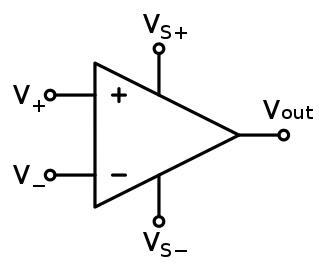
\includegraphics[width=0.3\textwidth]{images/op-amp_circuit_diagram.png}
		\caption{Circuit Diagram for an op-amp. Pins are labeled below\label{op-amp diagram}}
	\end{figure}

	\begin{center}
		\textbf{V\textsubscript{1}}	= Input voltage at non-inverting terminal

		\textbf{V\textsubscript{2}}	= Input voltage at inverting terminal

		\textbf{V\textsubscript{0}}	= Output Voltage
	\end{center}

	\textbf{(+)} = Non-inverting input point

	\textbf{(-)} = Inverting input terminal

	\textbf{+Vcc} = Positive Voltage Supply

	\textbf{-V$\epsilon\epsilon$} = Negative supply

	\textbf{Vid} = Diffrential input = (V\textsubscript{1} $-$ V\textsubscript{2})
	\vskip 0.7cm

	The power supply pins \textbf{+Vcc} and \textbf{-V$\epsilon\epsilon$} can also be labeled in different ways. As shown in \textbf{Figrue: \ref{op-amp diagram}}

	\subsection{Operation}

	The amplifier's differential inputs consist of a non-inverting input(+) with voltage V\textsubscript{+} an inverting input(\-) with Voltage V\textsubscript{-}; ideally the op-amp amplifies only the difference in voltage between the two, which is called the \textsf{differential input voltage}. The output voltage of the op-amp V\textsubscript{out} is given in the equation

	$\bgroup\Large{\textbf{V\textsubscript{out} = A\textsubscript{OL}(V\textsubscript{+} - V\textsubscript{-})}}\egroup{}$

	\begin{figure}[hbt!]
		\centering
		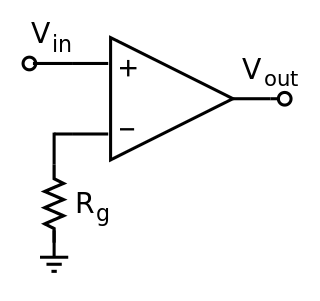
\includegraphics[width=0.3\textwidth]{images/op-amp without negative feedback.png}
		\caption{An op-amp without negative feedback}
	\end{figure}

	where A\textsubscript{OL} is the \textcolor{blue}{open-loop} gain of the amplifier (the term ``open-loop'' refers to the absence of a fedd-back loop from the output to the input)

	\subsection{Classification}

	Op-amps may be classified by their construction:

	\begin{itemize}
		\item discrete (built from individual \textcolor{blue}{transistors} or \textcolor{blue}{tubes/valves})
		\item IC (fabricated in an \textcolor{blue}{Integrated Circuit}) - most common
		\item hybrid
	\end{itemize}

	\subsection{Applications}

	\begin{wrapfigure}{R}{2.5in}
		\centering
		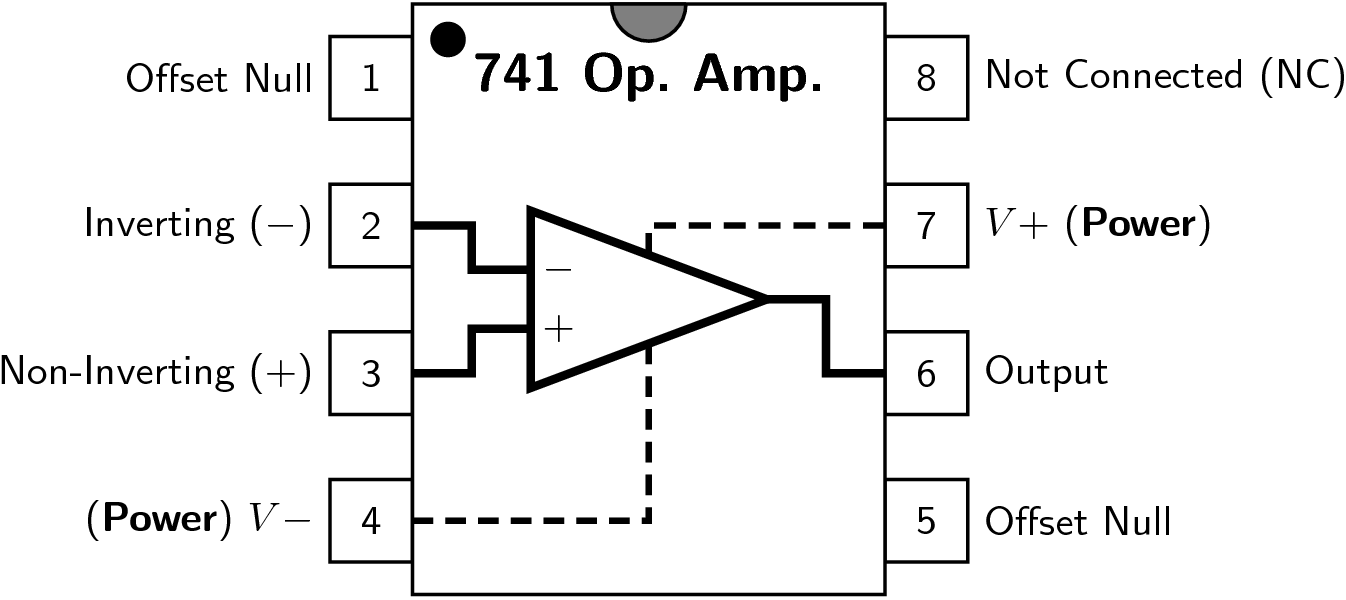
\includegraphics[width=2in]{images/741-type operational amplifier.png}
		\caption{\textcolor{blue}{DIP pinout} for 741-type operational amplifier}
	\end{wrapfigure}

	\subsubsection{Use in electronics system design}

	The use of op-amps as circuit blocks is much easier and clearer than specifying all their individual circuit elements(transistors, resistors, etc.), whether the amplifiers used are integrated or discrete circuits.

	Circuit design follows the same lines for all electronic circuits. A specification is drawn governing what the circuit is required to do, with allowable limits. For example, the gain may be required to be 100 times, with a tolerance of 5\% but drift of less than 1\% in a specified temperature range; the input impedence not less than one megohm; etc.

	\subsubsection{Other applications}

	\begin{itemize}
		\item audio- and video-frequency \textcolor{blue}{pre-amplifiers} and \textcolor{blue}{buffers}
		\item \textcolor{blue}{differential amplifiers}
		\item \textcolor{blue}{differentiators} and \textcolor{blue}{integrators}
		\item filters
		\item precision \textcolor{blue}{peak detectors}
		\item volatage and current \textcolor{blue}{regulators}
		\item analog calculators
		\item analog-to-digital convertors
		\item digital-to-analog convertors
		\item Voltage clamping
		\item oscillators and waveform generators
		\item clipper
		\item clamper(dc inserter or restorer)
		\item LOG and ANITLOG amplifiers
	\end{itemize}

	Most single, dual and quad op-amps available have a standardized pin-out which permits one type to be subsituted for another without writing changes.

	\clearpage

	% this here below is for other question

	\section{Explain IC 741}

	The short form of the operational amplifier is op-amp, is a one kind of solid state IC. The first operational amplifier is designed by \textbf{\textcolor{orange}{Fairchild Semiconductors}} in the year \textbf{\textcolor{orange}{1963}}.

	These ICs uses an exterior feedback to regulate its functions and these components are used as a multipurpose device in various electronic instruments. It consists of two inputs and two outputs, namely inverting and non-inverting terminals. The main intention of this 741 op amp is to strength AC \& DC signals and for mathematical operations. It's \textcolor{orange}{applications} mainly involves in filter, comparators, pulse generators, oscillators, etc.

	\subsection{IC 741 Operational Amplifier}

	The \textcolor{orange}{IC 741 operational amplifier} looks like a small chip. The representation of 741 IC op-amp is given below that comprises of eight pins. The most significant pins are \textbf{2, 3 and 6}, where pin 2 and 3 are pin 2 and 3 denote inverting \& non-inverting terminals and pin 6 denotes output voltage. The triangular form in the IC signifies an op-amp integrated circuit. The main function of this IC 741 is to do mathematical operations in various circuits. IC 741 op amp is made from various stages of transistor which commonly have three stages like differential i/p, a push-pull o/p and an intermediate gain stage. The differential op-amps \textcolor{orange}{comprises of a set of FETs} or BJTs.

	\begin{figure}[hbt!]
		\centering
		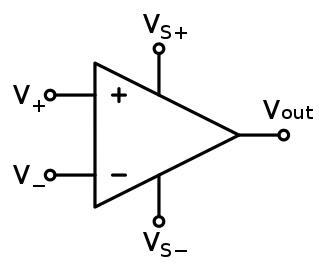
\includegraphics[width=0.4\textwidth]{images/op-amp_circuit_diagram.png}
		\caption{IC 741 Op-Amp}
	\end{figure}

	\subsection{Pin Diagram of IC 741 Op-Amp}

	The \textcolor{orange}{pin configuration of the IC 741 operational amplifier} is shown below. It comprises of eight pins where the function of each pin is discussed below.

	\begin{itemize}
		\item Pin-1 is Offset null.
		\item Pin-2 is Inverting (-) i/p terminal
		\item Pin-3 is a non-inverting (+) i/p terminal
		\item Pin-4 is -Ve voltage supply (Vcc)
		\item Pin-5 is offset null
		\item Pin-6 is the o/p voltage.
		\item Pin-7 is +ve voltage supply (+Vcc)
		\item Pin-8 is not connected.
	\end{itemize}

	\begin{figure}
		\centering
		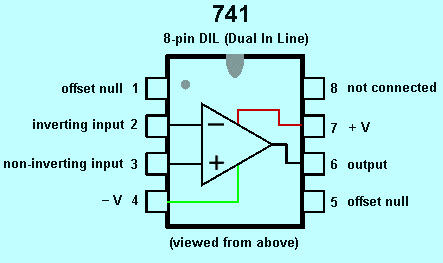
\includegraphics[width=0.4\textwidth]{images/Pin-Diagram-of-IC-741.jpg}
		\caption{Pin Diagram of IC 741 Op-Amp}
	\end{figure}

	The IC 741 operation amplifier is used in two methods such as an inverting(-) and a non inverting(+)

	\noindent Whenever any input voltage is applied at the \emph{\underline{non-inverting input terminal}}, the output voltage waveform phase does not change. (No phase shift is obtained between output and input) (0\degree or 360\degree phase shift is obtained)

	When input voltage is applied at inverting terminal, 180\degree phase shift is obtained at the output waveform.

	\clearpage
	% insert the image

	\section{Operation Amplifier Characterstics}

	In the table given below, ideal and practical characterstics of an op-amp are listed:

	\begin{center}
		\begin{table}[h]
			\begin{tabular}{ ||>{\bfseries} c || c || c || }
				\hline
				% there's a way to not do this
				\textbf{\underline{Parameter}} & \textbf{\underline{Ideal}} & \textbf{\underline{Practical}} \\
				\hline
				Op Amp & Vid & (V\textsubscript{1} $-$ V\textsubscript{2}) \\
				& (V\textsubscript{1} $-$ V\textsubscript{2}) & \nicefrac{1}{2}(V\textsubscript{1} $-$ V\textsubscript{2}) \\
				& & Ad -\textgreater very large, Ac -\textgreater very small \\
				\hline
				Gain & $\infty$(Ad) & Finite, Very large \\
				\hline
				Input resistance & $\infty$ & Very high \\
				Rin & & (in M$\Omega$) \\
				\hline
				Ouptut resistance & 0 & Very Small \\
				Rout & & \\
				\hline
				\nicefrac{Ad}{AC} = CMRR & $\infty$ & very large \\
				\hline
				Slow Rate & $\infty$ & Finite Very large \\
				\hline
				Bandwidth & $\infty$ & High/large \\
				\hline
				Input Offset voltage & 0 & Very low \\
				\hline
				Input Offset current & 0 & Very low \\
				\hline
		\end{tabular}
		\caption{characterstics of op-amp}
	\end{table}
\end{center}

\subsection{Block Diagram of an Op-Amp}

% Here insert block diagram image
\begin{figure}[hbt!]
	\centering
	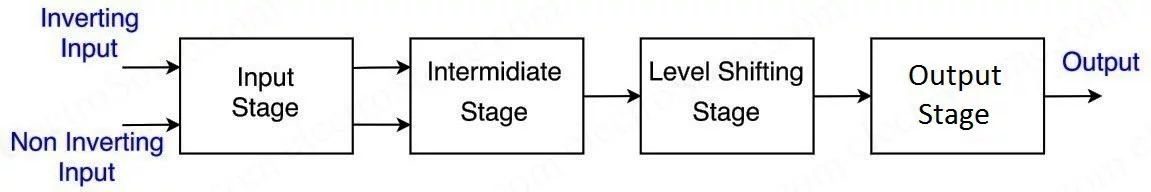
\includegraphics[width=1\textwidth]{images/op-amp block diagram.png}
	\caption{block diagram of an Op-Amp}
\end{figure}

\begin{enumerate}
	\item Dual \nicefrac{i}{p} balanced \nicefrac{o}{p} differential amplifier
	\item Dual \nicefrac{i}{p} unbalanced \nicefrac{o}{p} differential amplifier
	\item Emitter follows with constant current source
	\item Push-Pull Amplifier
\end{enumerate}

\clearpage

\section{Differential gain and Common-mode gain}

\subsection{Differential Amplifier\label{difamp}}

\begin{figure}[hbt!]
	\centering
	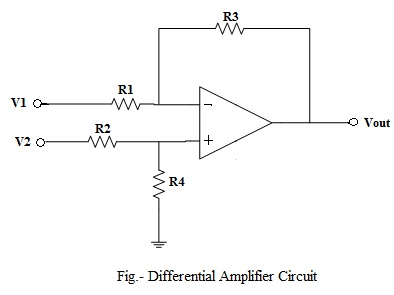
\includegraphics[width=0.5\textwidth]{images/Differential-amplifier-circuit.jpg}
	\label{Differential Amplifier circuit}
\end{figure}

The difference amplifier shown in the circuit is a combination of both inverting and non - inverting amplifiers. If the non-inverting terminal is connected to ground, the circuit operates an inverting amplifier and the input signal V\textsubscript{1} is amplified by (R\textsubscript{3}/R\textsubscript{1}).

Similarly, if the inverting input terminal is connected to ground, the circuit behaves as a non-inverting amplifier. With the inverting input terminal grounded, R\textsubscript{3} and R\textsubscript{1} function as the feedback components of a non-inverting amplifier.

Input V\textsubscript{2} is potentially divided across resistors R\textsubscript{2} and R\textsubscript{4} to give V\textsubscript{R4}, and then V\textsubscript{R4} is amplified by (R\textsubscript{3} + R\textsubscript{1})/R\textsubscript{1}.

With V\textsubscript{2} = 0,

\begin{center}
$V\textsubscript{O1} = -(R\textsubscript{3}/R\textsubscript{1})*V\textsubscript{1}$
\end{center}

With V\textsubscript{1} = 0,

\begin{center}
$V\textsubscript{R4} = \{R\textsubscript{4}/(R\textsubscript{2}+R\textsubscript{4})\}*V\textsubscript{2}$
\end{center}

\begin{center}
	and
\end{center}

\begin{center}
$V\textsubscript{02} = \{R\textsubscript{1}+(R\textsubscript{3}/R\textsubscript{1})\}*V\textsubscript{R4}$
\end{center}

Therefore,

\begin{center}
$V\textsubscript{02} = \{R\textsubscript{1}+(R\textsubscript{3}/R\textsubscript{1})\}*\{R\textsubscript{1}+(R\textsubscript{3}/R\textsubscript{1})\}*V\textsubscript{R4}$
\end{center}

If the input resistance are chosen such that, R\textsubscript{2} = R\textsubscript{1} and R\textsubscript{4} = R\textsubscript{3}, then

\begin{center}
$V\textsubscript{O2} = \{R\textsubscript{3}/R\textsubscript{1}\}*V\textsubscript{2}$
\end{center}

Now, according to superposition principle if both the input signals V\textsubscript{1} and V\textsubscript{2} are present, then the output voltage is

\begin{center}
$V\textsubscript{O} = V\textsubscript{O1} + V\textsubscript{O2}$
\end{center}

\begin{center}
$=\{-(R\textsubscript{3}/R\textsubscript{1}) * V\textsubscript{1}\} + \{R\textsubscript{3}/R\textsubscript{1}\}*V\textsubscript{2}$
\end{center}

Which results in,

\begin{center}
$V\textsubscript{0} = (\textsubscript{3}/R\textsubscript{1}) * \{V\textsubscript{2} - V\textsubscript{1}\}$
\end{center}

When the resistors R\textsubscript{3} and R\textsubscript{1} are of the same value, the output is the direct difference of the input voltages applied. By selecting R\textsubscript{3} greater than R\textsubscript{1}, the output can be made an amplified version of the difference of the input voltages.

\subsection{Differential Gain}

The differential gain of a difference amplifier \textbf{\ref{difamp}} is defined as the gain obtained at the output signal with respect to the difference in the input signals applied.

The output voltage of a difference amplifier is given as,

\begin{center}
	$V\textsubscript{O} = A\textsubscript{D}(V\textsubscript{1} - V\textsubscript{2})$
\end{center}

where, A\textsubscript{D} = -(R\textsubscript{3}/R\textsubscript{1}) is the differential gain of the amplifier.

\subsection{Common-mode gain}

A perfect operational amplifier amplifies only the voltage difference between its two inputs, completely rejecting all voltages that are common to both. However, the differential input stage of an operational amplifier is never perfect, leading to the amplification of these common voltages to some degree. The standard measure of this defect is called the common-mode rejection ratio (denoted CMRR). Minimization of common mode gain is usually important in non-inverting amplifiers (described below) that operate at high amplification.

\clearpage

\section{Input Impdence, Output Impedence, Offset Voltage}

\subsection{Input Impdence(Z\textsubscript{in})}

Input Impedance is defined as the input voltage by the \textcolor{orange}{input current}. The input impedance of an ideal op amp is $\infty$. That is there no current flowing in the input circuit. However, an ideal op amp has certain current flowing in the input circuit of the magnitude of few pico-amps to a few milli-amps.

\subsection{Output Impedance(Z\textsubscript{out})}

Output impedance is defined as the ratio of the output voltage to the input current. The output impedance of an ideal op amp is 0, however, real \textcolor{orange}{op amps} have an output impedance of 10-20 k$\Omega$. An \textcolor{orange}{ideal op amp} behaves like a perfect \textcolor{orange}{voltage source} delivering current without any internal losses. The internal resistance reduce the voltage available to the load.

\subsection{Offset Voltage(V\textsubscript{io})}

The offset voltage of an \textcolor{orange}{ideal op amp} is zero, which means that the output voltage will be zero if the difference between the inverting and non-inverting terminal is zero. If both the terminals are grounded, the output voltage will be zero. But real \textbf{op amps} have an offset voltage.

\end{document}
